\documentclass{article}
\usepackage{tikz}
\usepackage{verbatim}
%%%>


\usetikzlibrary{calc,backgrounds}

\usetikzlibrary{bayesnet}
%\usepackage[active,tightpage]{preview}

\begin{document}

%\begin{preview}
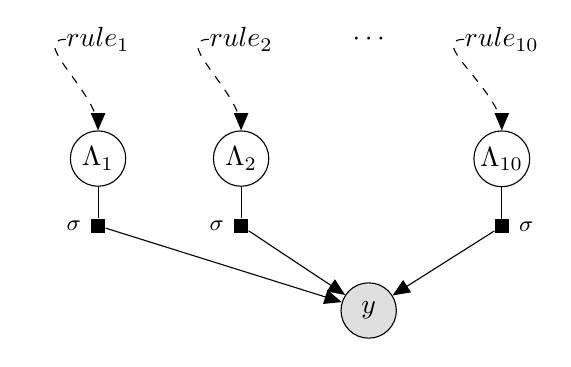
\begin{tikzpicture}

\node[const](r1){$rule_1$};
\node[const,right=of r1](r2){$rule_2$};
\node[const,right = of r2](cdot){$\cdots$};
\node[const,right=of cdot](r10){$rule_{10}$};
\node[latent,below= of r1](l1){$\Lambda_1$};
\node[latent,below= of r2](l2){$\Lambda_2$};
\node[latent,below= of r10](l10){$\Lambda_{10}$};

  \draw [->,dashed] (r1) to [out=180,in=90] (l1);
    \draw [->,dashed] (r2) to [out=180,in=90] (l2);
      \draw [->,dashed] (r10) to [out=180,in=90] (l10);
      
      \node[obs, below = 3 of cdot](y){$y$};
      
       \factor[below= of l1] {l1-y} {left:$\sigma$} {l1} {y} ;
              \factor[below= of l2] {l2-y} {left:$\sigma$} {l2} {y} ;
                     \factor[below= of l10] {l10-y} {right:$\sigma$} {l10} {y} ;

\end{tikzpicture}
%\end{preview}

\end{document}
%\endpgfgraphicnamed

%%% Local Variables: 
%%% mode: tex-pdf
%%% TeX-master: "example"
%%% End: 